\documentclass[a4paper,11pt]{article}

% ------- Encoding & idioma -------
\usepackage[utf8]{inputenc}
\usepackage[T1]{fontenc}
\usepackage[spanish,es-tabla,es-noshorthands]{babel}

% ------- Layout -------
\usepackage[a4paper,top=2cm,bottom=2cm,left=2.2cm,right=2.2cm]{geometry}
\usepackage{parskip}
\setlength{\parindent}{0pt}

% ------- Tipografía -------
\usepackage{lmodern}
\usepackage{microtype}

% ------- Color & secciones -------
\usepackage{xcolor}
\definecolor{azulOscuro}{HTML}{1F3A5F}
\definecolor{azulMedio}{HTML}{2A5B8D}
\definecolor{grisFondo}{HTML}{F4F6FA}
\definecolor{grisLinea}{HTML}{CCCCCC}

\usepackage{titlesec}
\titleformat{\section}{\normalfont\Large\bfseries\color{azulOscuro}}{\thesection.}{0.5em}{}
\titleformat{\subsection}{\normalfont\large\bfseries\color{azulMedio}}{\thesubsection.}{0.5em}{}
\titlespacing*{\section}{0pt}{16pt}{8pt}
\titlespacing*{\subsection}{0pt}{10pt}{4pt}

% ------- Figuras & tablas -------
\usepackage{graphicx}
\usepackage{float}
\graphicspath{{figuras/}}
\usepackage{caption}
\captionsetup{font=small,labelfont={bf,color=azulMedio},textfont=it}

\usepackage{booktabs}
\usepackage{array}
\usepackage{tabularx}
\usepackage{colortbl}

\newcommand{\hd}[1]{\textbf{\textcolor{white}{#1}}}
\newcommand{\filaCabecera}{\rowcolor{azulOscuro}}

% ------- Hipervínculos -------
\usepackage[hidelinks]{hyperref}
\hypersetup{
  pdftitle={Tarea 1 - Introduccion a la Ciencia de Datos},
  pdfauthor={Pilar Busquets, Joaquin Campo},
  pdfsubject={Maestria CDAA, FING (2026)},
}

\setcounter{secnumdepth}{0}

\begin{document}

\begin{titlepage}
  \centering
  \vspace*{3cm}

  {\LARGE\bfseries\color{azulOscuro} Tarea 1\par}
  \vspace{0.4cm}
  {\Large\bfseries Cargado, Limpieza y Conteo de Palabras\par}

  \vspace{2.5cm}

  {\large Introducción a la Ciencia de Datos\par}
  \vspace{0.3cm}
  {\itshape\color{gray} Maestría en Ciencia de Datos y Aprendizaje Automático\par}
  {\itshape\color{gray} Facultad de Ingeniería, UdelaR\par}

  \vfill

  {\large\bfseries Autores\par}
  \vspace{0.3cm}
  {\large Pilar Busquets\par}
  {\large Joaquin Campo\par}

  \vfill

  {\large 2026\par}
  \vspace{2cm}
\end{titlepage}

\section{Parte 1. Cargado y Limpieza de Datos}

\subsection{A. Exploración inicial y selección de medios}

El dataset contiene \textbf{30.213} artículos en 12 columnas. La inspección con \texttt{df.info()} y \texttt{df.isna().sum()} muestra varios problemas de calidad.

\textbf{Datos faltantes por columna.}

\begin{center}
\begin{tabular}{lr}
\toprule
\filaCabecera \hd{Columna} & \hd{\% faltantes}\\
\midrule
author      & 37,75\% \\
section     & 33,87\% \\
article     &  3,89\% \\
url         &  0,47\% \\
publication &  0,47\% \\
\bottomrule
\end{tabular}
\end{center}

\texttt{author} y \texttt{section} tienen aproximadamente un tercio de faltantes. Como no se usan como variables para el análisis posterior, se decide dejarlas sin imputar. \texttt{article} tiene 3,89\% de faltantes y se reemplaza por un string vacío en la limpieza para conservar el título. Los 141 registros sin \texttt{publication} (0,47\%) se eliminan al filtrar por los cinco medios principales.

\textbf{Problemas adicionales de calidad.} 

En el \texttt{df.info()} se ve que las columnas que corresponden a variables temporales (\texttt{date}, \texttt{year}, \texttt{month}, \texttt{day}) están guardadas como strings. \texttt{date} además tiene formatos inconsistentes (\texttt{2018-02-02} y \texttt{2017-04-03 00:00:00}). En el código se convierten con \texttt{pd.to\_datetime(date, format="mixed", errors="coerce")} y ninguna fila queda como \texttt{NaT}.

\textbf{Distribución por medio.}

\begin{center}
\begin{tabular}{lr}
\toprule
\filaCabecera \hd{Medio} & \hd{Cantidad de artículos}\\
\midrule
Reuters            & 9.431 \\
The New York Times & 2.840 \\
CNBC               & 2.623 \\
The Hill           & 2.349 \\
People             & 1.528 \\
\bottomrule
\end{tabular}
\end{center}

Quedan \textbf{18.771} artículos si se filtra por el top 5 de medios con más artículos. La distribución es desbalanceada ya que Reuters tiene 9.431 artículos (49,7\%), People 1.528 (8,1\%).

\subsection{B. Visualización temporal}

\begin{figure}[h]
  \centering
  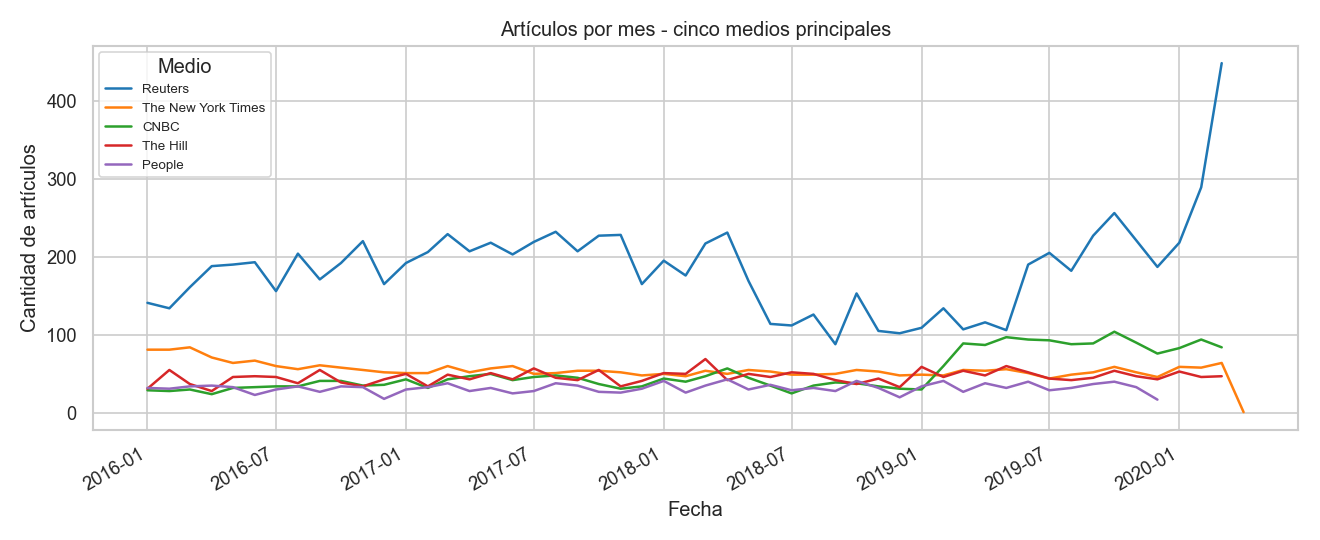
\includegraphics[width=0.95\textwidth]{01_serie_temporal.png}
  \caption{Cantidad de artículos por mes para los cinco medios principales.}
\end{figure}

The New York Times, The Hill, CNBC y People oscilan entre 30 y 70 artículos por mes en todo el dataset. Reuters está claramente por encima, entre 150 y 250 mensuales.

El pico más claro es Reuters en marzo y abril de 2020, que pasa de unos 200 artículos por mes a cerca de 450, coincidente con el inicio de la pandemia. Antes hay una caída de Reuters en julio y agosto de 2018 (de $\sim$230 a $\sim$100 artículos por mes) sin explicación a primera vista. CNBC presenta un crecimiento más abrupto a comienzos de 2019 que después se estabiliza en aproximadamente 100 artículos por mes de mitad de año en adelante. También se denota que llegando al 2020, se notan algunas anomalías. The People no muestra publicaciones. The New York Times decae abruptamente y Reuters se dispara. Como es cerca de la cota superior del intervalo, se entiende que puede ser producto de cómo fueron muestreados los datos y no características del dataset.

\subsection{C. Limpieza de texto y conteo de palabras}

La función \texttt{clean\_text} normaliza los artículos para que un conteo por palabra no diferencie entre formas como \emph{President}, \emph{president.} y \emph{president,}. Sobre la versión provista, se agregan las siguientes transformaciones, en orden:

\begin{itemize}
  \item \textbf{Convertir a minúsculas}.
  \item \textbf{Reemplazar URLs por espacio} mediante una expresión regular (\texttt{https?://...} y \texttt{www\textbackslash....}). Las URLs introducen tokens muy específicos (dominios, paths) que son fuertísimos identificadores del medio.
  \item \textbf{Normalizar tipografía no-ASCII}: comillas tipográficas curvas, guiones largos y elipsis se sustituyen por espacio.
  \item \textbf{Eliminar signos de puntuación}. A la lista original se agregan paréntesis, llaves, corchetes, punto y coma, barras, asteriscos, signos de porcentaje y otros ASCII usados en notas periodísticas.
  \item \textbf{Eliminar dígitos} con \texttt{\textbackslash d+}. No aportan al vocabulario y reducen la dispersión causada por fechas y cifras económicas.
  \item \textbf{Colapsar espacios múltiples} a uno.
\end{itemize}

La función se aplica sobre \texttt{FullText = title + ". " + article}. El resultado queda en la columna \texttt{CleanText}.

\subsection{D. Elección de campos de texto}

La elección entre cuerpo, título o ambos depende de la aplicación. Si se busca una caracterización rápida de las noticias, el título puede ser suficiente porque concentra la información editorial más visible, aunque entrega poco texto por artículo. Si interesa aprovechar el contenido completo, el cuerpo aporta más términos y contexto, pero en este corpus deja sin texto al 3,89\% de los artículos que no tienen \texttt{article}. Para este trabajo se usa la combinación \texttt{title + ". " + article}: permite mantener esos artículos mediante su título y, en los demás casos, suma el contexto del cuerpo. El punto y el espacio se eliminan en la limpieza, así que no afectan el conteo.

\subsection{E. Pistas que identifican al medio de prensa}

Se busca en el corpus patrones que den indicios de a qué medio corresponden de manera directa: nombre del medio, dominio web, formas de cierre de artículo.

\begin{center}
\begin{tabular}{lrrr}
\toprule
\filaCabecera \hd{Medio} & \hd{Art. con pista} & \hd{\% del medio} & \hd{Apariciones}\\
\midrule
The Hill           & 2.335 & 99,4\% & 3.677 \\
Reuters            & 8.763 & 92,9\% & 27.291 \\
CNBC               &   907 & 34,6\% &  1.832 \\
The New York Times &   646 & 22,7\% &  1.156 \\
People             &    51 &  3,3\% &     58 \\
\bottomrule
\end{tabular}
\end{center}

99,4\% de los artículos de The Hill y 92,9\% de los de Reuters mencionan al propio medio. Esto está dado por la estructura del propio artículo, ya que analisandolo se nota que vienen de las firmas (\texttt{(Reuters)}, \emph{Reporting by ...}) y estructura de cómo cierran el artículo. CNBC y The New York Times también tienen un gran porcentaje (34,6\% y 22,7\%), People apenas 3,3\%. En el top de palabras de la Figura 2 esto reaparece como \emph{reuters}, \emph{reporting}, \emph{editing} en Reuters y \emph{hill}, \emph{thehill} en The Hill.

\subsection{F. Restricción por sección o por período}

Restringir el análisis ayudaría a aislar las diferencias de estilo del efecto del tema (que People se distinga porque ``escribe distinto'' y no sólo porque ``cubre celebridades''). Las dos opciones tienen problemas.

\emph{Por sección.} \texttt{section} tiene 33,87\% de faltantes y las etiquetas no son comparables entre medios (Reuters etiqueta \emph{Healthcare}, CNBC \emph{Health and Science}). Habría que mapear taxonomías a mano antes de cualquier filtro.

\emph{Por período.} Es más simple. La Figura 1 sugiere quedarse en 2017-2019 y dejar fuera el pico de la pandemia en Reuters en 2020 y la cola incompleta del dataset. Se pierde volumen y, además, el período más interesante.

\clearpage

\section{Parte 2. Conteo de Palabras y Visualizaciones}

\subsection{A. Palabras más frecuentes por medio}

Se tokeniza \texttt{CleanText} por espacios, se descartan tokens de longitud menor o igual a 2 y se aplica una lista de stopwords (NLTK en inglés más un pequeño conjunto frecuente en periodismo como \emph{said}, \emph{would}, \emph{also}, \emph{year}). Se reportan las 15 palabras más frecuentes por medio posterior a ese filtrado.

\begin{figure}[h]
  \centering
  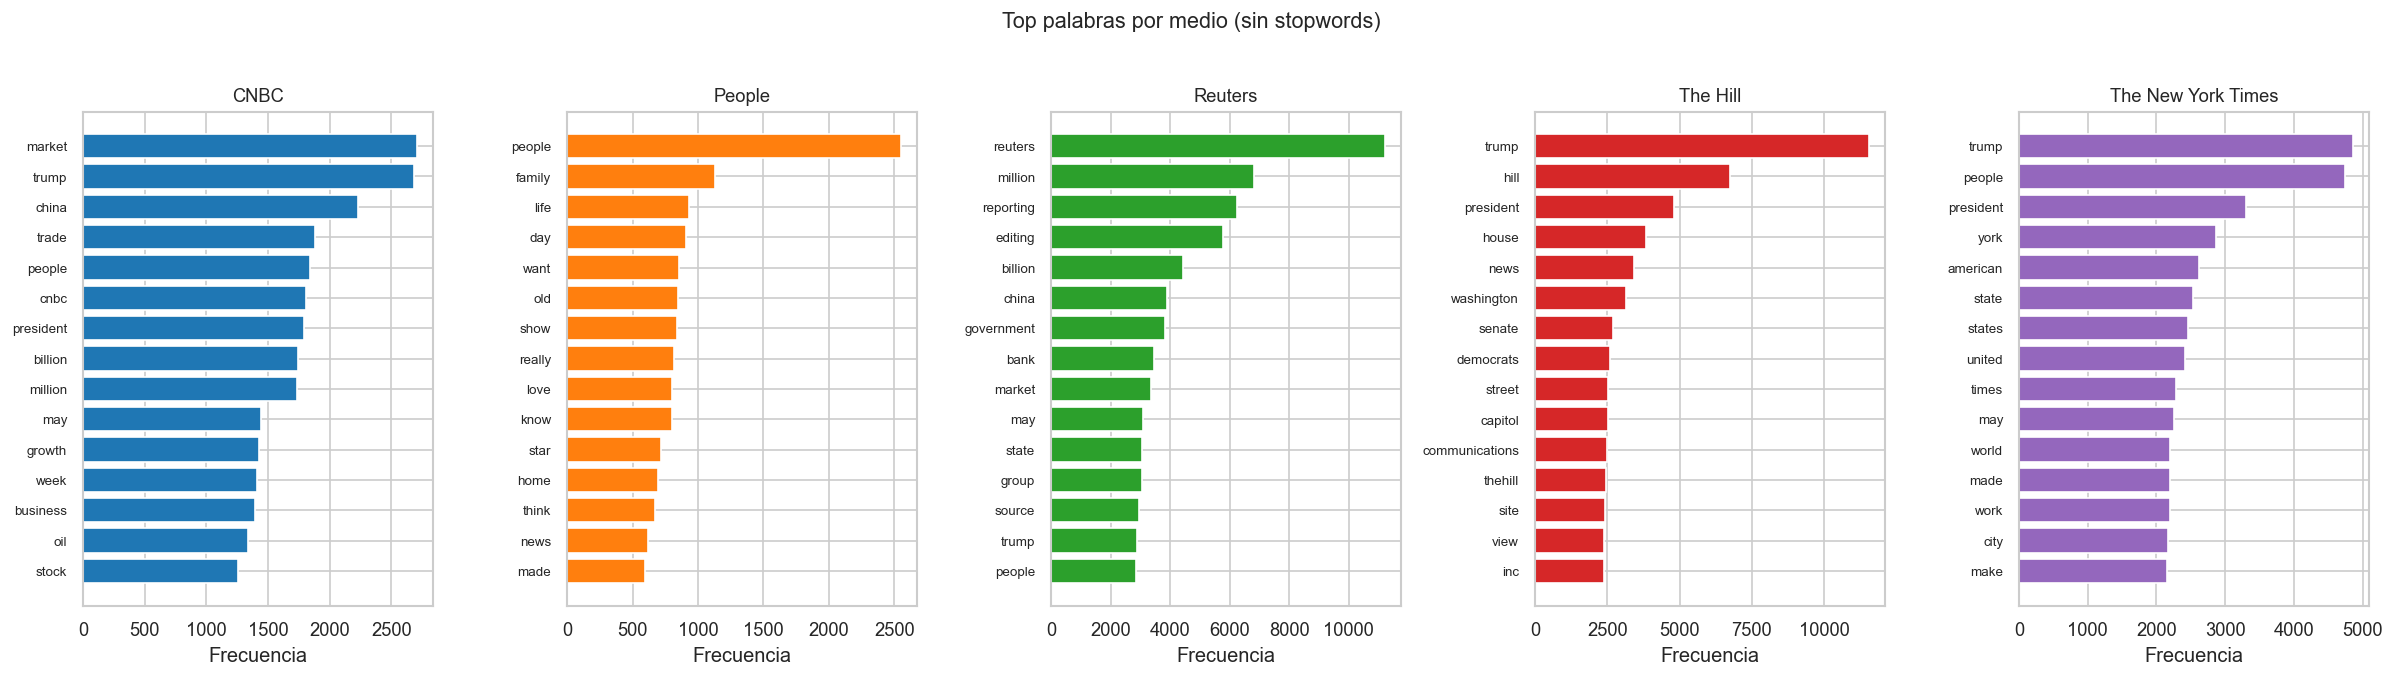
\includegraphics[width=\textwidth]{02a_top_palabras.png}
  \caption{Top 15 palabras por medio, luego de remover stopwords.}
\end{figure}

Diferencias temáticas: vocabulario económico en CNBC y Reuters (\emph{market}, \emph{trade}, \emph{billion}), político en The Hill y The New York Times (\emph{trump}, \emph{president}, \emph{house}, \emph{senate}), entretenimiento y vida personal en People (\emph{family}, \emph{life}, \emph{love}, \emph{star}). En paralelo, las pistas de 1.E reaparecen en los rankings: \emph{reuters}, \emph{reporting}, \emph{editing} en Reuters, \emph{hill}, \emph{thehill} en The Hill, \emph{cnbc} en CNBC, \emph{york}, \emph{times} en The New York Times, \emph{people} encabezando People.

Ideas para esta visualización:

\begin{itemize}
  \item TF-IDF en lugar de frecuencia bruta, para resaltar palabras distintivas de un medio frente a los otros cuatro.
  \item Bigramas y trigramas, para capturar conceptos compuestos por más de una palabra \emph{white house}, \emph{wall street}, \emph{new york times}.
  \item Visualizar palabras exclusivas de cada medio.
\end{itemize}

\subsection{B. Medios con mayor cantidad de palabras}

Se calcula, por medio, el total de palabras en \texttt{CleanText}, la cantidad de artículos y el promedio por artículo.

\begin{center}
\begin{tabular}{lrrr}
\toprule
\filaCabecera \hd{Medio} & \hd{Total palabras} & \hd{Artículos} & \hd{Promedio / art.}\\
\midrule
The New York Times & 2.623.472 & 2.840 & 924 \\
Reuters            & 2.606.519 & 9.431 & 276 \\
The Hill           & 1.373.555 & 2.349 & 585 \\
CNBC               & 1.240.543 & 2.623 & 473 \\
People             &   649.707 & 1.528 & 425 \\
\bottomrule
\end{tabular}
\end{center}

\begin{figure}[H]
  \centering
  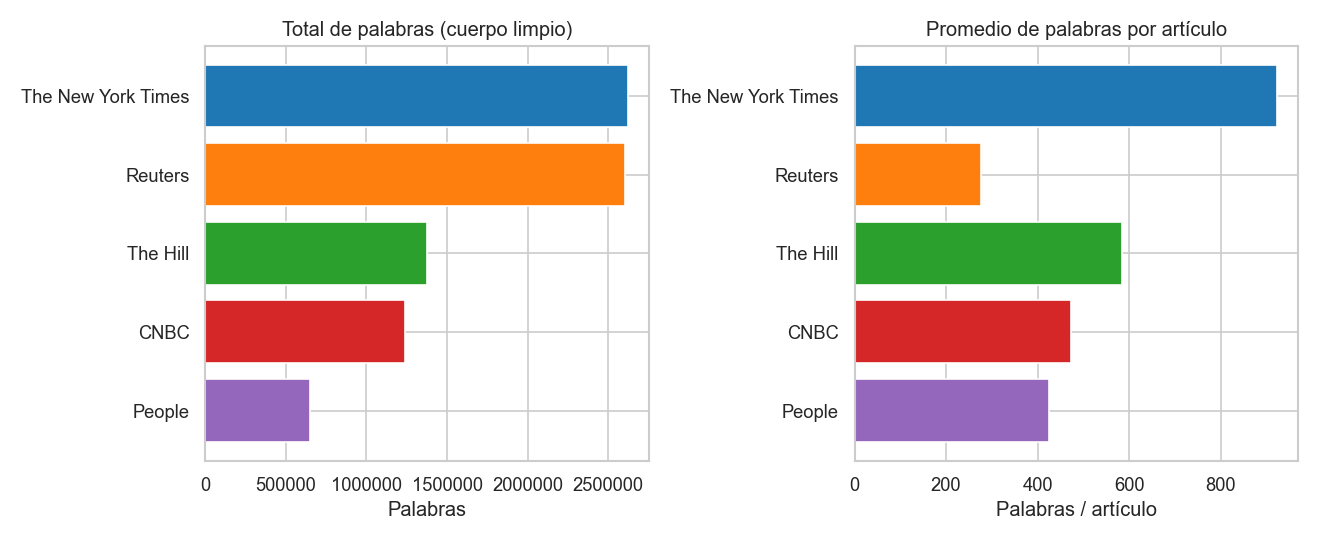
\includegraphics[width=0.95\textwidth]{02b_palabras_por_medio.png}
  \caption{Total de palabras por medio y promedio por artículo.}
\end{figure}

The New York Times y Reuters tienen aproximadamente la misma cantidad de palabras en total ($\sim$2,6 millones de palabras). Sin embargo, haciendo un análisis más profundo se puede notar que por razones opuestas: The New York Times son pocos artículos largos (924 palabras de promedio) y Reuters son muchos cortos (276). El total por sí solo sugiere volumen comparable y da a entender que ambos medios producen volumen comparable. Por eso la Figura 3 separa total y promedio por artículo en paneles distintos.

\subsection{C. Matriz de menciones entre medios}

Se cuentan, en cada artículo del medio $i$, las ocurrencias de referencias explícitas al medio $j$ (nombre y dominio principal). El resultado se muestra como mapa de calor en la Figura 4 (diagonal omitida) y como grafo dirigido en la Figura 5.

\begin{figure}[h]
  \centering
  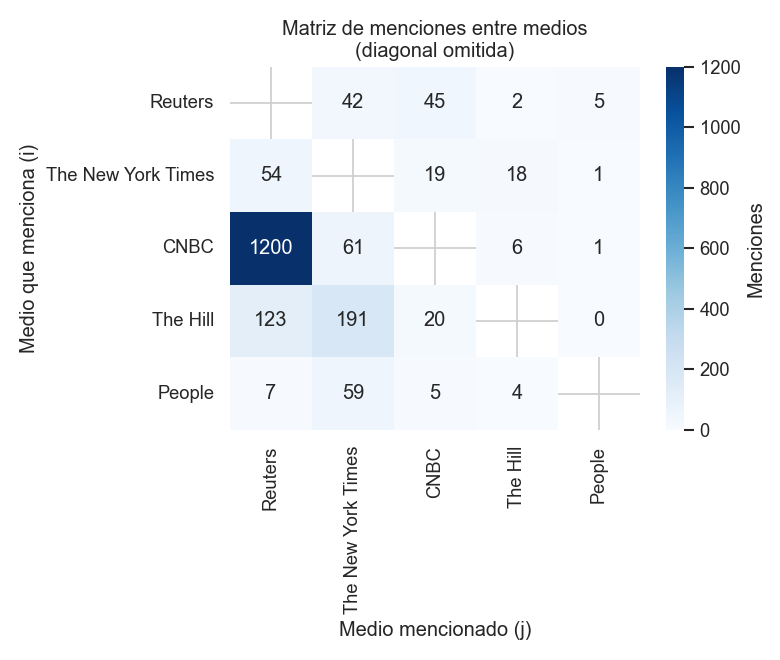
\includegraphics[width=0.78\textwidth]{02c_matriz_menciones.png}
  \caption{Mapa de calor de la matriz de menciones (diagonal omitida).}
\end{figure}

\begin{figure}[h]
  \centering
  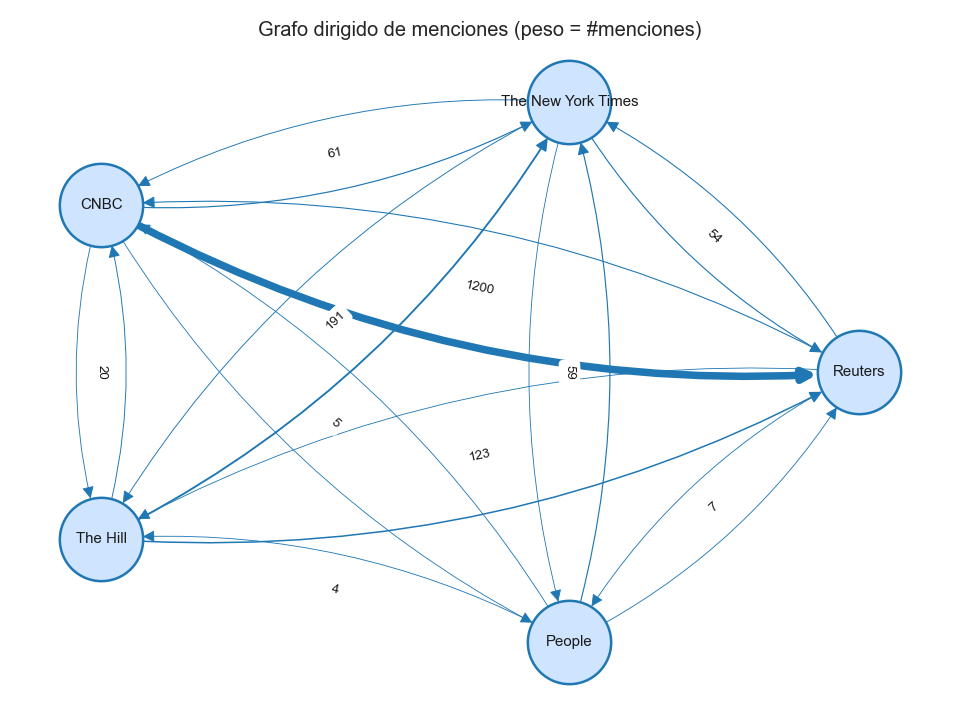
\includegraphics[width=0.88\textwidth]{02c_grafo_menciones.png}
  \caption{Grafo dirigido de menciones (ancho de arista proporcional al peso).}
\end{figure}

El peso más alto es CNBC hacia Reuters (1.200 menciones). Esto da a entender que debería existir algun tipo de relación entre estos dos medios. Buscamos en internet y encontramos acuerdos de provisión de noticias y datos entre Reuters y NBC, dueña de CNBC, explicando las observaciones. Después aparecen The Hill hacia The New York Times (191) y The Hill hacia Reuters (123). The New York Times menciona a Reuters 54 veces. People aparece sólo con 59 menciones a The New York Times.


\subsection{D. Preguntas propuestas}

\textbf{1. ¿Se puede separar a los medios en un espacio vectorial del texto?} Vectorizar los artículos con TF-IDF o embeddings preentrenados, aplicar reducción de dimensionalidad (PCA, t-SNE, UMAP) y visualizarlos graficamente.

\textbf{2. ¿Qué variables explican mejor las diferencias observadas entre medios?} Construir variables como longitud del artículo, cantidad de menciones a otros medios, frecuencia de entidades, proporción de citas y temas dominantes. Luego evaluar su importancia con correlaciones, información mutua o modelos interpretables para identificar qué características separan realmente a los medios.

\textbf{3. ¿Cómo cambian los patrones de cobertura a lo largo del tiempo?} Agrupar los artículos por fecha y estudiar series temporales de volumen de publicación, temas tratados y menciones entre medios. Esto permite detectar tendencias, cambios de agenda o períodos donde ciertos medios aumentan su actividad sobre un tema.

\textbf{4. ¿Qué tan similares son los medios según los temas que cubren?} Aplicar modelado de tópicos o clustering sobre representaciones vectoriales de los artículos y comparar la composición temática de cada medio. La idea es medir si los medios se diferencian por estilo, por agenda temática o por ambos factores. También se podría usar este clusterizado para imputar valores faltantes en la columna de \texttt{section}.
\end{document}
